\documentclass[11pt,a4paper]{article}
\usepackage[latin1]{inputenc}
\usepackage{amsmath}
\usepackage{amsfonts}
\usepackage{amssymb}
\usepackage{graphicx}
\usepackage{longtable}
\usepackage{tabularx}
\usepackage{enumitem}
\usepackage{url}
\usepackage[margin=0.8in]{geometry}
\usepackage[toc,page]{appendix}
\usepackage{etoolbox}
\usepackage{morefloats}
\usepackage{multirow}
\usepackage[hidelinks]{hyperref}
\usepackage{float} % Allows putting an [H] in \begin{figure} to specify the exact location of the figure
\usepackage{verbatim}
\usepackage{listings}
\usepackage[usenames,dvipsnames]{color}

\graphicspath{{img/}}

\patchcmd{\thebibliography}{\section*}{\subsection}{}{}

% Table padding
\renewcommand{\arraystretch}{1.5}

\begin{document}

\begin{titlepage}

\begin{center}

\includegraphics[width=0.5\textwidth]{img/University_Logo}\\

\textsc{\LARGE Swansea University }\\[0.5cm]
\textsc{\large MEng Computing }\\[2cm]

{ \huge \bfseries Group Project CS-M04}\\[0.2cm]
\textsc{\large Team Structure, Methodology, Requirements and Specifications}\\[1.5cm]

\begin{minipage}{0.4\textwidth}
\begin{flushleft}

\emph{Authors:}\\
Adam \textsc{Barrell} {\scriptsize \emph{(632975)}} \\
Thomas \textsc{Milner} {\scriptsize \emph{(637755)}} \\
Lewis \textsc{Hancock} {\scriptsize \emph{(xxxxxx)}} \\
Christopher \textsc{Lewis} {\scriptsize \emph{(xxxxxx)}} \\

\end{flushleft}
\end{minipage}
\begin{minipage}{0.4\textwidth}
\begin{flushright}

\emph{Supervisor:}\\
Parisa \textsc{Eslambolchilar}

\end{flushright}
\end{minipage}\\[1.3cm]

{\today}
\end{center}

\end{titlepage}

\newpage 

\tableofcontents

\newpage
\section{Introduction}
This document, White Rock Digital Trails: Interim Document, shall guide the reader through the current state of the project. This includes the design of user interfaces, implementation of features and project management tasks such as a schedule update and analysis of any risks the project has encountered.
\subsection{Purpose}
The document aims to inform the reader of all progress made on the project since the last document. It was originally created as part of an MEng Computing degree at Swansea University, under the supervision of Parisa Eslambolchilar, for the White Rock team (TODO:CITE). The document is also suitable for third parties interested in the development of White Rock Digital Trails, subject to permission from the authors. The document acts a follow-up document to the previously written Milestone 1: (TODO: find name and cite).
\subsection{Overview}
%- Outline of Document (what we cover in the document).

\section{Technology Choices}
\subsection{Android}

\subsection{Eclipse}

\subsection{Android Devices}

%- What APIs, Libraries, IDEs etc we are using, compared with other options we had. Argue our choices.

\section{Project Progress}
%- THIS IS THE OVERVIEW SECTION
%- Show the subsystem designs and explain the current structure of the project. 
%- Possible to move the risk management and schedule sections up here if people feel it reads better. Depends how big those sections get.

\subsection{Database}

%- Why do we need a database, what data will it store?
A relational database has been created to store persistent data for the web portal and Android application.
The database will store data relating to entities such as walks, way points, users and media locations.

%- How was the database designed?
A table has been created for each entity or concept that requires persistent storage.
%- How was the database be generated from this model?
%- How will the database be exposed if not directly?
%- Where will the database be hosted?
%- What applications will consume data from this database?
%- How does it's design conform to the requirements?
%- Describe the relationships (one-one) (one-many) (many-many)

\begin{figure}[H]
\centering
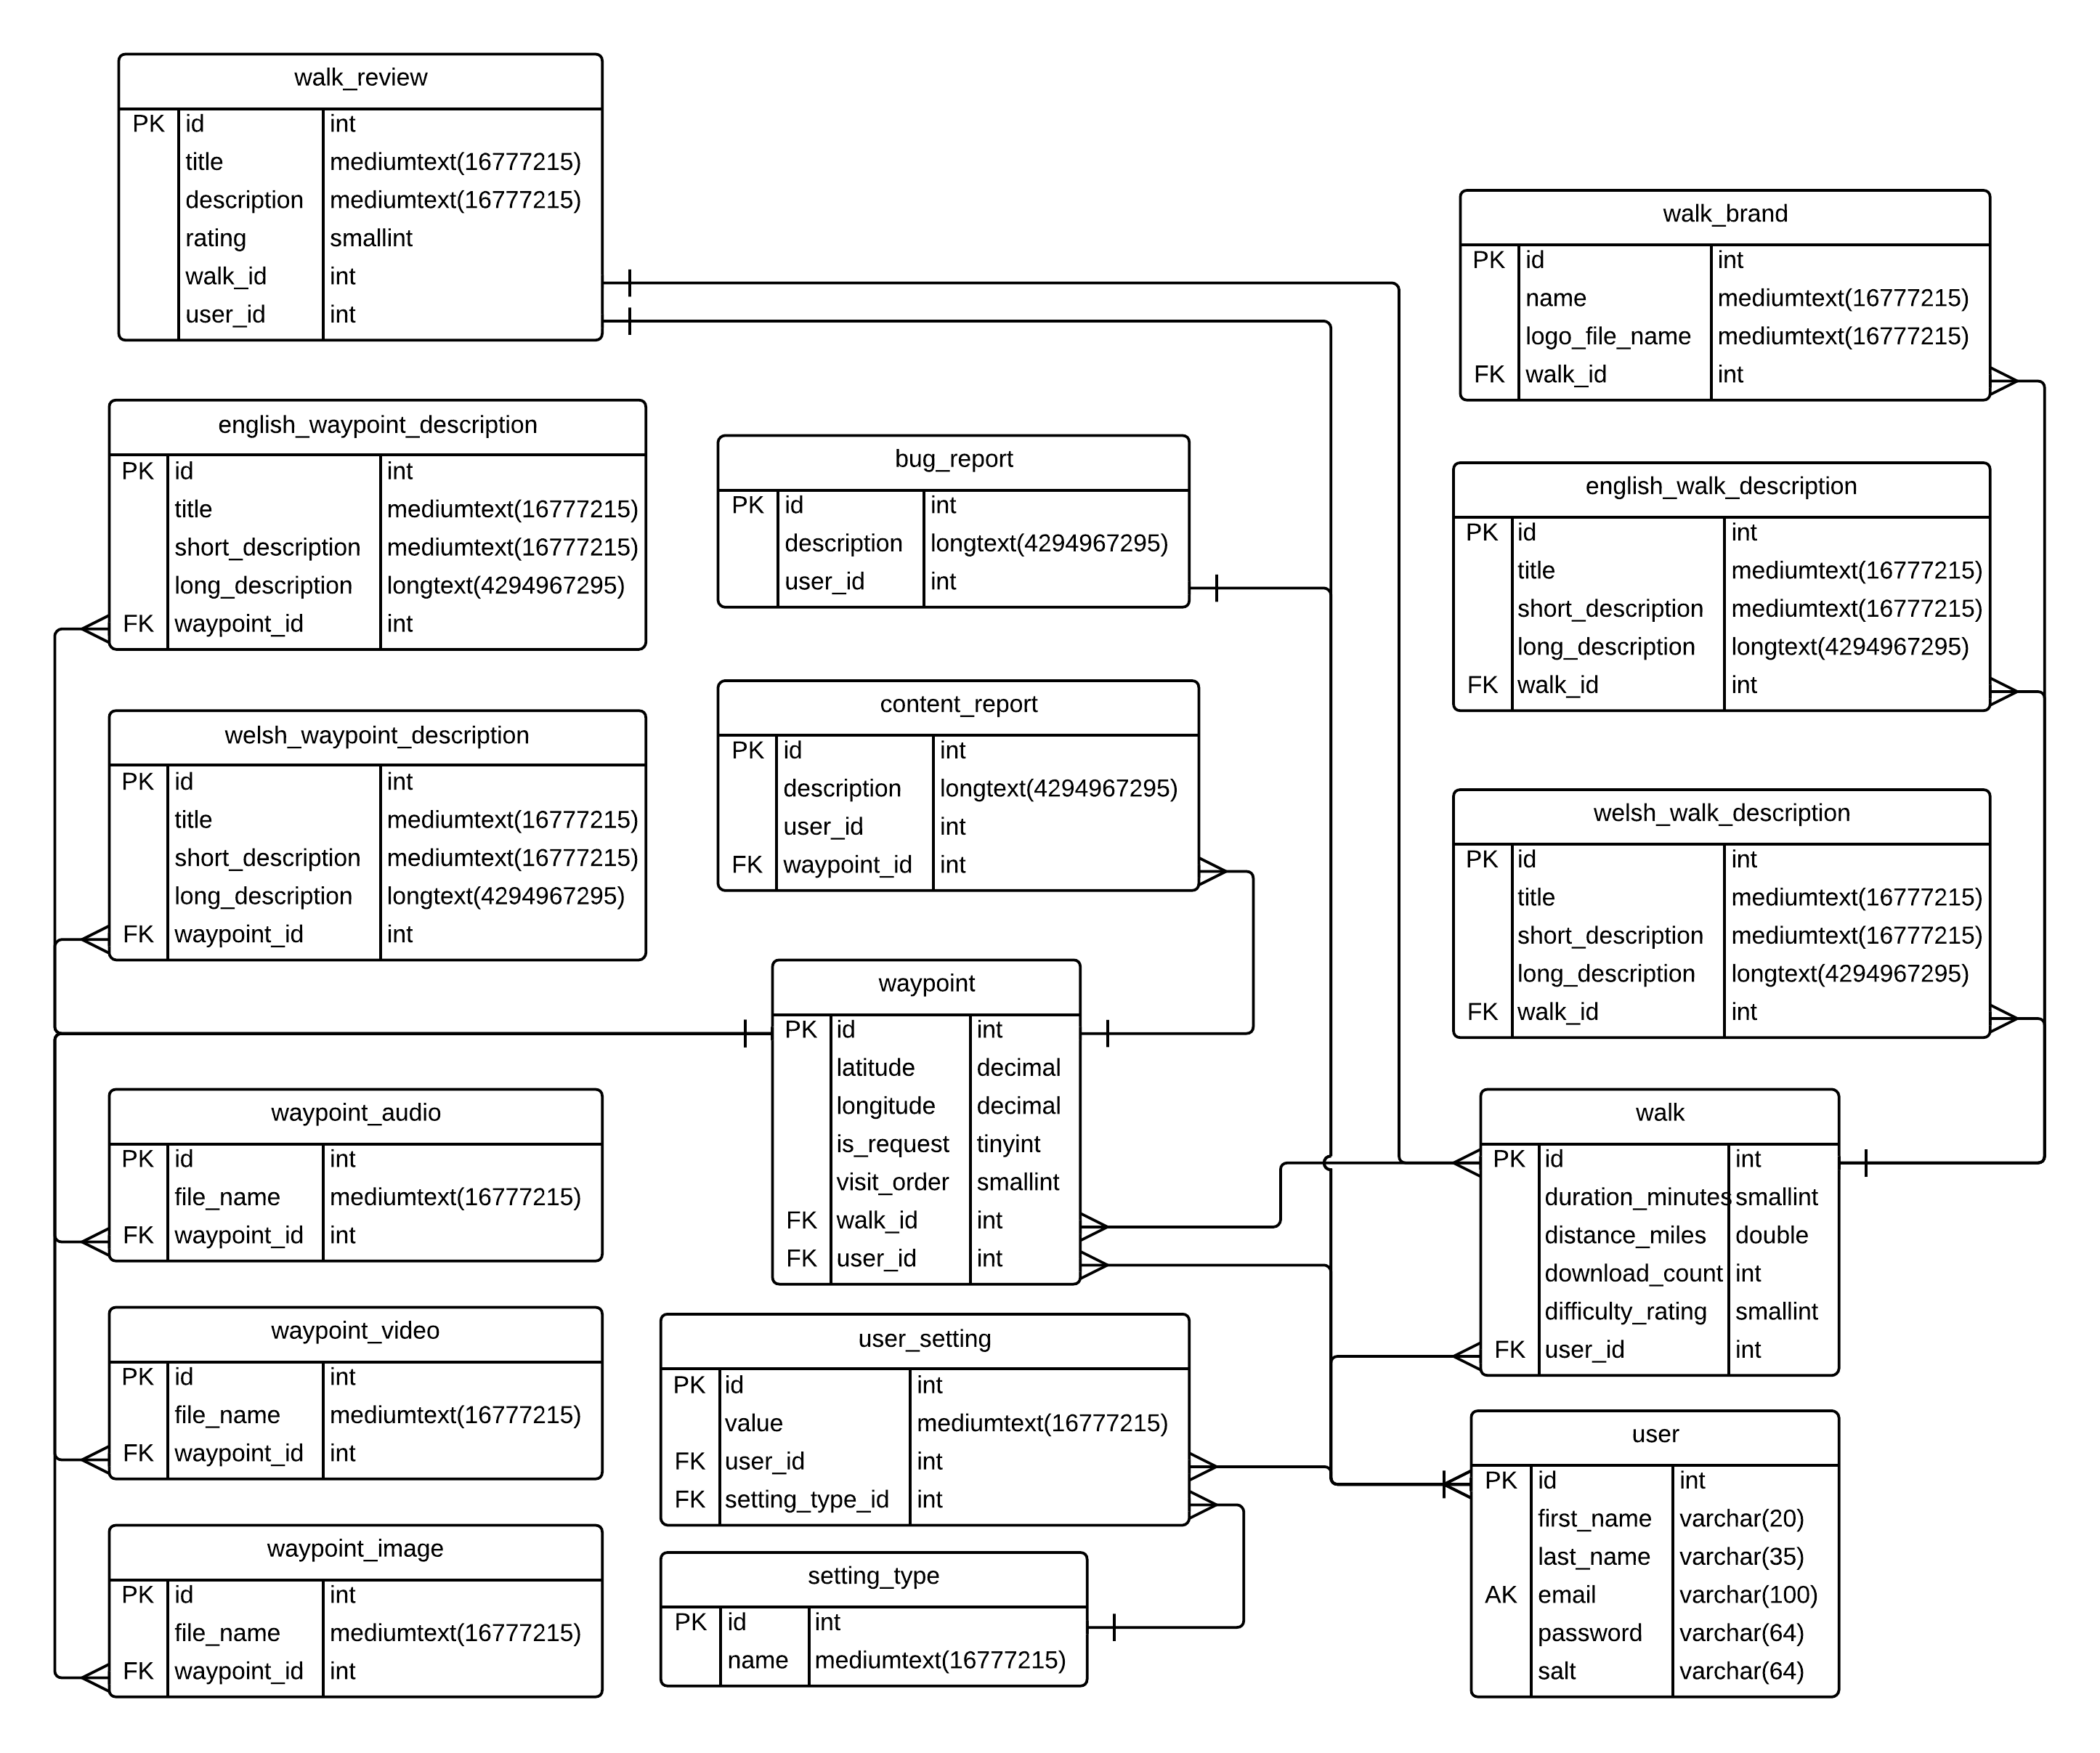
\includegraphics[angle=90, width=1\linewidth]{./img/DatabaseSchema}
\caption{Schema of the White Rock Trails relational database.}
\label{fig:DatabaseSchema}
\end{figure}


\subsection{User Interfaces}
%- Heuristic Evaluations on similar products
%-- Explain how we are doing the evaluation blahblah nielsen etc.
%-- List of tasks for evaluators to complete (we should really ALL be involved in doing the evaluations).
%-- Problems found when completing each task
%- Our prototype UI 1
%-- show how it meets reqs, how heuristics helped design.
%-- Heuristics on this etc.
%- Our prototype UI 2
%-- show it meets reqs, how heuristics helped design.
%-- Heuristics
%- repeat as necessary.

\section{Android Application Progress}
\lstset{language=Java,
keywordstyle=\color{red},
commentstyle=\color{OliveGreen},
showstringspaces=false}
The development of the Android application is progressing well and has been unaffected by risks, both expected and unexpected. To achieve the goals of the project, the application has to be capable of saving and loading data to and from a local database, which will then synchronise with the remote database - this is achieved via a content provider, seen in Section~\ref{sec:contentprovier}; the client also requested Google Maps be implemented, the progress of which can be seen in Section~\ref{sec:googlemaps}; as the application allows users to log-in and personalise their experience an authentication system has been created, seen in Section~\ref{sec:authorisation}. Finally, fragments and activities have been created to control the flow of the program, along with relevant layouts and graphics, which can be seen in Section~\ref{sec:fragments}. All of these systems, when completed, will meet the requirements shown in Section 4.1.2 of the Milestone 1 document. %TODO: Cite
\subsection{Content Provider}
\label{sec:contentprovier}
The content provider provides valuable functionality when synchronising with the server and allowing for other applications to, potentially, access the application's database. It consists of four components. Firstly, there is the DbSchema class, this interface class contains all of the SQL used to create the table and constants such as table names. Next comes the DatabaseHandler class, an extension of the Android SQLiteOpenHelper class, which creates the database and contains the strategy for deleting and upgrading the database; it is also responsible for opening and closing connections to the database. The WhiteRockContract class provides an API for foreign applications to access available data, without this the content provider does not achieve anything. Finally, there is the WhiteRockContentProvider class itself, this class is responsible for inserting, deleting, updating and querying the database.

\subsubsection{Database Schema}
The DbSchema class is an interface which is strictly used for referencing constants, such as table names, and strings containing the SQL used to create each table in the database. Example code can be seen in Listing~\ref{lst:dbSchema}.

\begin{lstlisting}[captionpos=b, caption=DbSchema Snippet, label=lst:dbSchema, frame=single]
	// Example code snippet from DbSchema.java
	
	String VIEW_WAYPOINT_WITH_ENGLISH_DESCR = "waypoint_and_english";
	
	String CREATE_TABLE_WALK = 
			"CREATE TABLE `walk` (" 
			+"_id INTEGER PRIMARY KEY AUTOINCREMENT ,"
			+"duration_minutes INT,"
			+"distance_miles REAL,"
			+"download_count INT,"
			+"difficulty_rating INT,"
			+"user_id INT"
			+")";
	
	String CREATE_TABLE_WALK_BRAND = 
			"CREATE TABLE `walk_brand` ("
			+"_id INTEGER PRIMARY KEY AUTOINCREMENT ,"
			+"name TEXT,"
			+"logo_file_name TEXT,"
			+"walk_id INT"
			+")";
\end{lstlisting}

\subsubsection{DatabaseHandler}
Responsible for creating, deleting and upgrading the database, as well as opening and closing connections, the DatabaseHandler class is vital for both maintaining the database and interfacing with it.

Listing~\ref{lst:dbHandler} provides a snippet of the code used during the creation of a DatabaseHandler instance and how it uses the DbSchema to create the database.

\begin{lstlisting}[captionpos=b, caption=DatabaseHandler Snippet, label=lst:dbHandler, frame=single]
	public DatabaseHandler(Context context) {
		super(context, DB_NAME, null, DB_VERSION);
		
		// Find the correct path based on Android version.
		if (android.os.Build.VERSION.SDK_INT >= Build.VERSION_CODES.JELLY_BEAN_MR1) {
			DB_PATH = context.getApplicationInfo().dataDir + "/databases/";
		} else {
			DB_PATH = "/data/data/" + context.getPackageName() + "/databases/";
		}
		Log.d(TAG,"DB Path is: " + DB_PATH+DB_NAME);
		Log.d(TAG, "Version Number: " + android.os.Build.VERSION.SDK_INT);
		this.mContext = context;
	}

	@Override
	public void onCreate(SQLiteDatabase db) {
		Log.d(TAG, "CREATING");
		// create User tables
		db.execSQL(DbSchema.CREATE_TABLE_USER);
		db.execSQL(DbSchema.CREATE_TABLE_SETTING_TYPE);
		db.execSQL(DbSchema.CREATE_TABLE_USER_SETTINGS);
		
		// Create Walk Tables
		db.execSQL(DbSchema.CREATE_TABLE_WALK);
		db.execSQL(DbSchema.CREATE_TABLE_WALK_BRAND);
		db.execSQL(DbSchema.CREATE_TABLE_WALK_REVIEW);
		db.execSQL(DbSchema.CREATE_TABLE_ENGLISH_WALK_DESCR);
		db.execSQL(DbSchema.CREATE_TABLE_WELSH_WALK_DESCR);
	}
\end{lstlisting}

\subsubsection{WhiteRockContract}
The WhiteRockContract class is the API which all applications, including this one, must use to access the ContentProvider. The class itself is relatively simple, providing constant values for the Authority and Content URI's required to access the data. The content provider accesses data from the database by being passed a URI in the format content://authority//path\_to\_type. In this implementation the authority is ``uk.ac.swan.digitaltrails'' the path\_to\_type variable points to a table name, such as ``walk''. An example of this, for the ``bug\_report'' table, can be seen in Listing~\ref{lst:contract}.

\begin{lstlisting}[captionpos=b, caption=WhiteRockContract Snippet, label=lst:contract, frame=single]
public class WhiteRockContract {
	
	public static final String AUTHORITY = "uk.ac.swan.digitaltrails";
	public static final Uri CONTENT_URI = Uri.parse("content://" + AUTHORITY);


	/**
	 * Constants for Bug Report table.
	 * @author Lewis Hancock
	 *
	 */
	public static final class BugReport implements ReportColumns {
		public static final Uri CONTENT_URI = Uri.withAppendedPath(
				WhiteRockContract.CONTENT_URI, "bug_report");
	
		public static final String CONTENT_TYPE = ContentResolver.CURSOR_DIR_BASE_TYPE +
				"vnd.uk.ac.swan.digitaltrails.bug_report";
		
		public static final String CONTENT_TYPE_DIR = ContentResolver.CURSOR_ITEM_BASE_TYPE +
				"vnd.uk.ac.swan.digitaltrails.bug_report";
		
		public static final String SORT_ORDER_DEFAULT = ID + " ASC";
		
		public static final String[] PROJECTION_ALL = {ID, DESCRIPTION, USER_ID};

	}
	// rest of code omitted
}
\end{lstlisting}


\subsubsection{WhiteRockContentProvider}
The WhiteRockContentProvider class is where all of the components come together. A URIMatcher is created to ensure that the correct data is accessed, according to the content URI passed. Based on the call to the content provider (insert, update, delete, query), the URI passed is matched via the URIMatcher and the operation carried out on the correct data in the correct table. Examples of each operation can be seen in Listing~\ref{lst:contentprovider}.

\begin{lstlisting}[captionpos=b, caption=WhiteRockContentProvider Snippet, label=lst:contentprovider, frame=single]
	private static UriMatcher buildUriMatcher() {
		final UriMatcher matcher = new UriMatcher(UriMatcher.NO_MATCH);
		final String authority = WhiteRockContract.AUTHORITY;
		matcher.addURI(authority, "walk", WALK_LIST);
		matcher.addURI(authority, "walk/#", WALK_ID);
		matcher.addURI(authority, "english_walk_description", ENGLISH_WALK_DESCR_LIST);
		matcher.addURI(authority, "english_walk_description/#", ENGLISH_WALK_DESCR_ID);
		matcher.addURI(authority, "welsh_walk_description", WELSH_WALK_DESCR_LIST);
		matcher.addURI(authority, "welsh_walk_description/#", WELSH_WALK_DESCR_ID);
	}
	
		@Override
		public boolean onCreate() {
			Context context = getContext();
			mDbHandler = new DatabaseHandler(context);
			return true;
		}
		
		@Override
		public int delete(Uri uri, String selection, String[] selectionArgs) {
			SQLiteDatabase db = mDbHandler.getWritableDatabase();
			int deleteCount = 0;
			String idStr;
			String where;
			
			switch (URI_MATCHER.match(uri)) {
			case WALK_LIST:
				deleteCount = db.delete(DbSchema.TABLE_WALK, selection, selectionArgs);
				break;
			case WALK_ID:
				idStr = uri.getLastPathSegment();
				where = WhiteRockContract.Walk._ID + " = " + idStr;
				if (!TextUtils.isEmpty(selection)) {
					where += " AND " + selection;
				}
				deleteCount = db.delete(DbSchema.TABLE_WALK, where, selectionArgs);
				break;
				// Rest of code omitted.
			}
			return deleteCount;
		}
		
		@Override
		public Uri insert(Uri uri, ContentValues values) {
			SQLiteDatabase db = mDbHandler.getWritableDatabase();
			long id = 0;
			switch (URI_MATCHER.match(uri)) {
			case WALK_LIST:
				id = db.insert(DbSchema.TABLE_WALK,
							  null,
						      values);
				db.close();
				return getUriForId(id, uri);
			case WAYPOINT_LIST:
				id = db.insert(DbSchema.TABLE_WAYPOINT,
							  null,
							  values);
				db.close();
				Log.d(TAG, "Attempting insert into waypoint table");
				return getUriForId(id, uri);
				
				// Rest of code omitted
			}
		}
		
		@Override
		public Cursor query(Uri uri, String[] projection, String selection, String[] selectionArgs,
				String sortOrder) {
			SQLiteDatabase db = mDbHandler.getReadableDatabase();
			SQLiteQueryBuilder builder = new SQLiteQueryBuilder();
			String queryString;
			boolean useAuthorityUri = false;
			switch (URI_MATCHER.match(uri)) {
			case WALK_LIST:
				builder.setTables(DbSchema.TABLE_WALK);
				if (TextUtils.isEmpty(sortOrder)) {
					sortOrder = WhiteRockContract.Walk.SORT_ORDER_DEFAULT;
				}
				break;
			case WALK_ID:
				builder.setTables(DbSchema.TABLE_WALK);
				builder.appendWhere(WhiteRockContract.Walk._ID + " = " + uri.getLastPathSegment());
				break;
				// rest of code omitted
			}
			Log.d(TAG, builder.getTables());
			Cursor cursor = builder.query(db, projection, selection, selectionArgs, null, null, sortOrder);
			if (useAuthorityUri) {
				cursor.setNotificationUri(getContext().getContentResolver(), WhiteRockContract.CONTENT_URI);
			} else {
				cursor.setNotificationUri(getContext().getContentResolver(), uri);
			}
			return cursor;
		}
		
		@Override
		public int update(Uri uri, ContentValues values, String selection, String[] selectionArgs) {
	
			SQLiteDatabase db = mDbHandler.getWritableDatabase();
			int updateCount = 0;
			String idStr;
			String where;
	
			switch(URI_MATCHER.match(uri)) {
			case WALK_LIST:
				updateCount = db.update(DbSchema.TABLE_WALK, values, selection, selectionArgs);
				break;
			case WALK_ID:
				idStr = uri.getLastPathSegment();
				where = WhiteRockContract.Walk._ID + " = " + idStr;
				if (!TextUtils.isEmpty(selection)) {
					where += " AND " + selection;
				}
				updateCount = db.update(DbSchema.TABLE_WALK, values, where, selectionArgs);
				break;
				// rest of code omitted.
			}
			return updateCount;
		}
	
\end{lstlisting}

\subsubsection{Using the Content Provider}
The content provider is currently being used, in conjunction with a CursorLoader, to query the database for walk names to choose a walk and, when a walk has been chosen, the waypoint details of that walk. The CursorLoader is an asynchronous loader, allowing data to be loaded in a different thread than the User Interface thread. This is great for loading the user interface whilst the data is loading. All the relevant code for loading data, in this example the titles of each walk and their details, can be seen in Listing~\ref{lst:walkListFragment}.

\begin{lstlisting}[captionpos=b, caption=WalkListFragment Snippet, label=lst:walkListFragment, frame=single]

public class WalkListFragment extends ListFragment 
	implements LoaderCallbacks<Cursor>, OnQueryTextListener {

	// Non-relevant code omitted.

	static String [] WALK_SUMMARY_PROJECTION = {WhiteRockContract.EnglishWalkDescriptions._ID, WhiteRockContract.EnglishWalkDescriptions.TITLE, WhiteRockContract.EnglishWalkDescriptions.WALK_ID };
	
	@Override
	public void onActivityCreated(Bundle savedInstanceState) {
		super.onActivityCreated(savedInstanceState);
		
		//setHasOptionsMenu(true);
		setEmptyText("No Walks");	//TODO load this from resource.
		mAdapter = new SimpleCursorAdapter(getActivity(), mLayout, null,
					new String[] {WhiteRockContract.EnglishWalkDescriptions.TITLE },
					new int[] {android.R.id.text1}, 0);	
		setListAdapter(mAdapter);
		setListShown(false);
		// Load the data!
		getLoaderManager().initLoader(0, null, this);
	}

	
	@Override
	public Loader<Cursor> onCreateLoader(int id, Bundle args) {
		Uri baseUri;
		if (mCurFilter != null) {
			baseUri = Uri.withAppendedPath(WhiteRockContract.CONTENT_URI, Uri.encode(mCurFilter));
		} else {
			baseUri = WhiteRockContract.EnglishWalkDescriptions.CONTENT_URI;
		}
		
		String select = "((_id))";
		return new CursorLoader(getActivity(), baseUri, WALK_SUMMARY_PROJECTION, select, null, WhiteRockContract.EnglishWalkDescriptions.WALK_ID + " COLLATE LOCALIZED ASC");
	}

	@Override
	public void onLoadFinished(Loader<Cursor> loader, Cursor data) {
		mAdapter.swapCursor(data);
		
		if (isResumed()) {
			setListShown(true);
		} else {
			setListShownNoAnimation(true);
		}
		
	}

	@Override
	public void onLoaderReset(Loader<Cursor> arg0) {
		mAdapter.swapCursor(null);
	}
}
\end{lstlisting}

All of the code (and more) in the above sections results in the screens and interactions seen in Figures~\ref{fig:walkListFragment} and~\ref{fig:googleContentLoader} being available in the application at the time of writing. This code is now completed, unless it becomes clear that we need access to other areas of the database.

\begin{figure}[H]
\centering
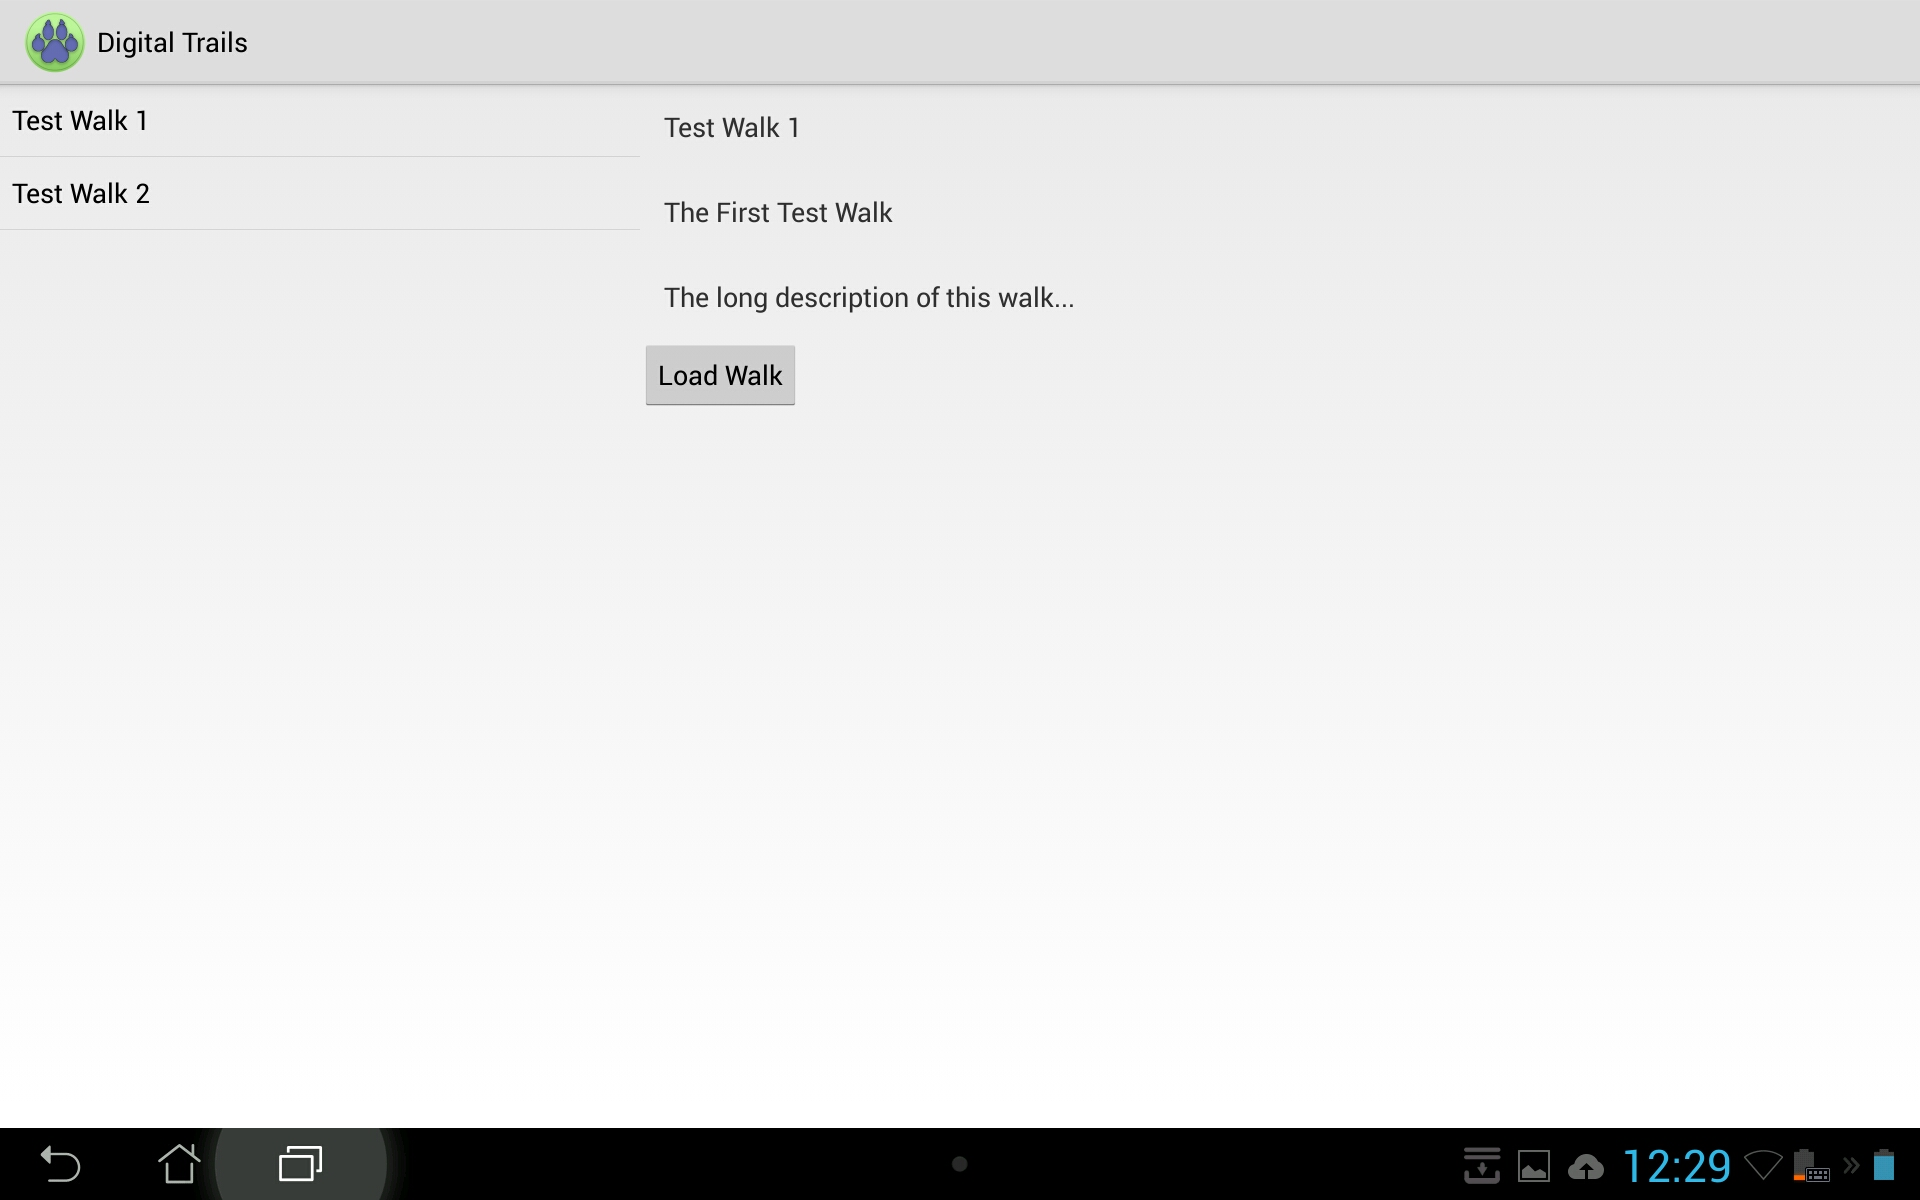
\includegraphics[angle=90, width=.5\linewidth]{walkListFragment.jpg}
\caption{Screenshot of WalkListFragment Fragment loading walk details from the database.}
\label{fig:walkListFragment}
\end{figure}


\begin{figure}[H]
\centering
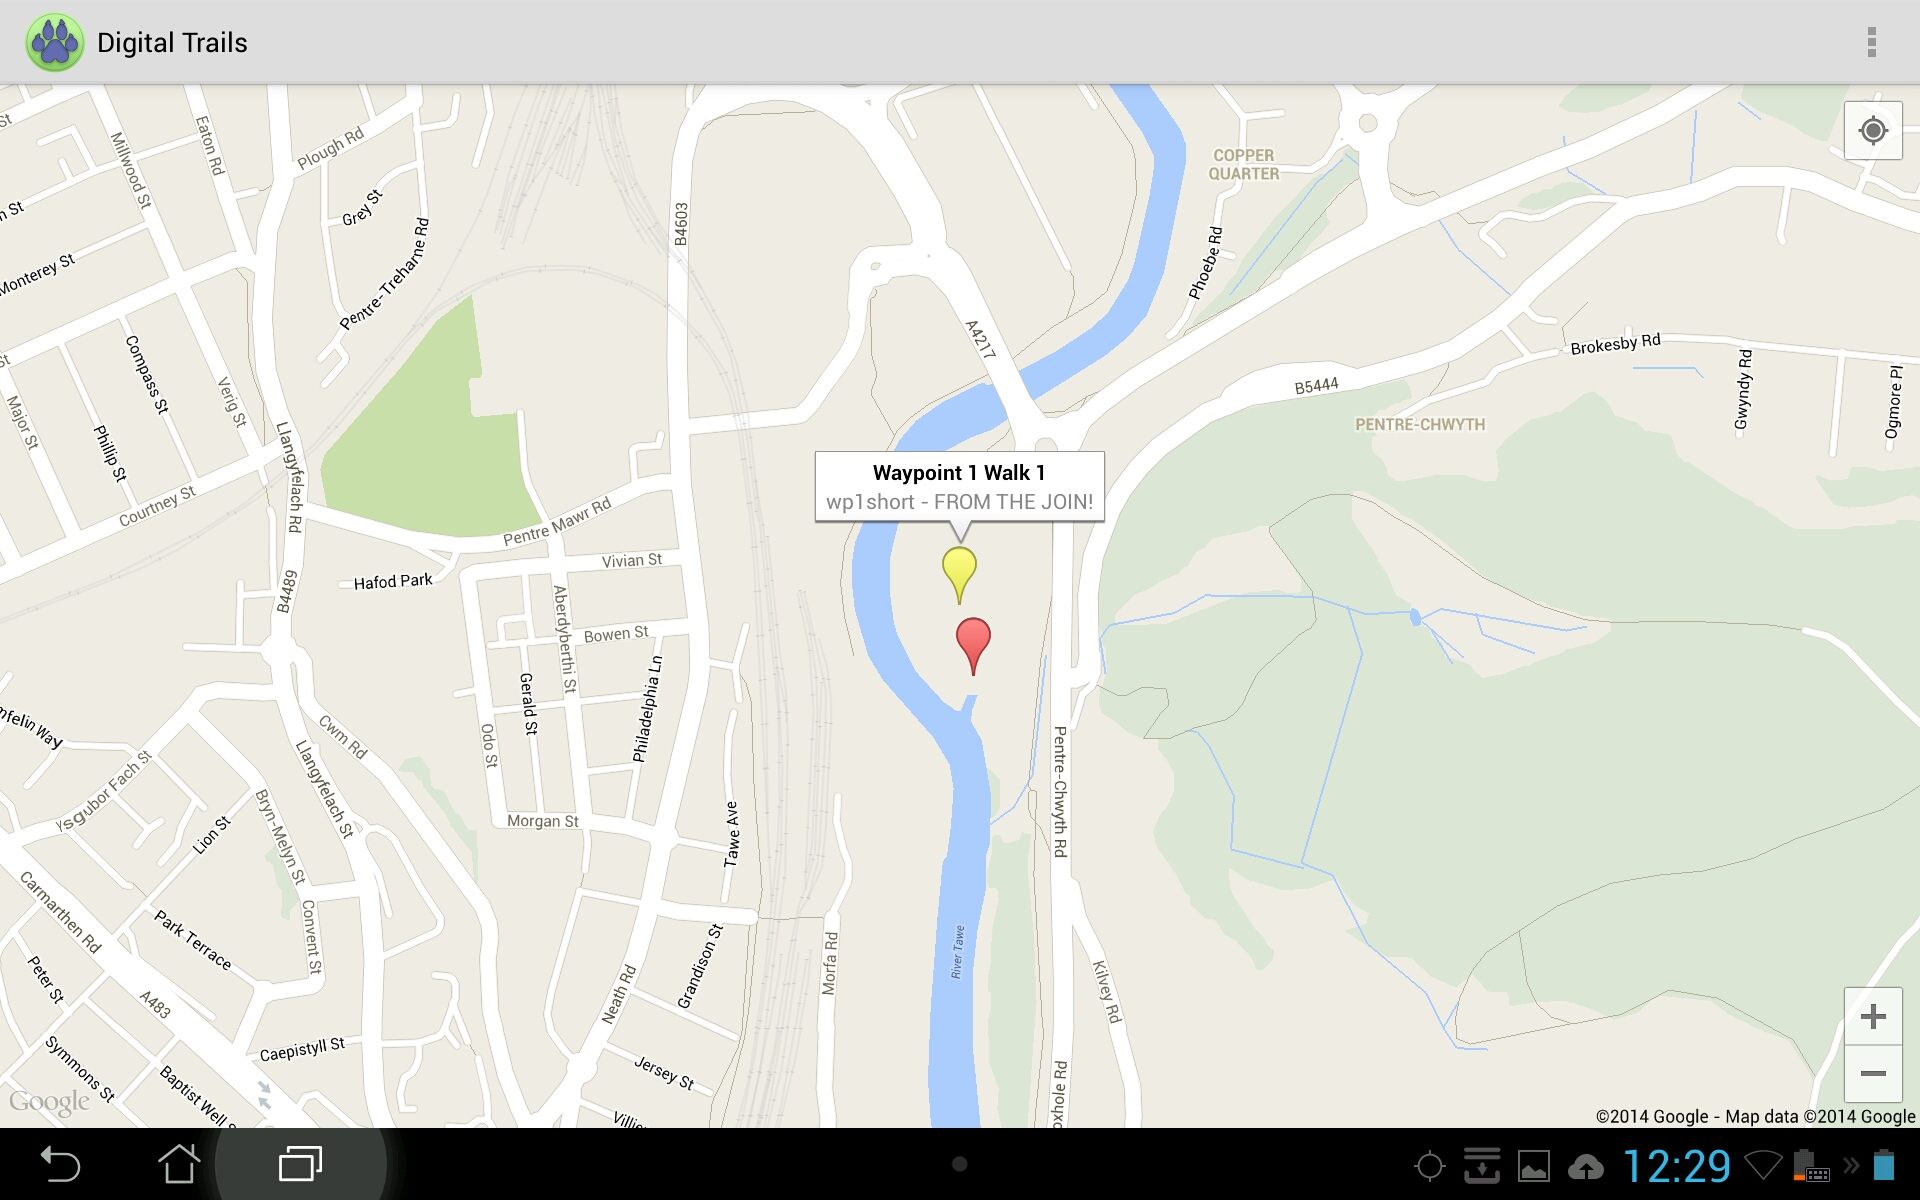
\includegraphics[angle=90, width=.6\linewidth]{googleMapsContentLoader.jpg}
\caption{Screenshot of the MapActivity displaying waypoint details from the database.}
\label{fig:googleContentLoader}
\end{figure}


\subsection{Google Maps}
\label{sec:googlemaps}
Currently the Google Maps API has been integrated at a basic level. The user can select a walk and the correct data will be displayed on the Map, with tappable waypoint markers. After tapping a marker a small information area (InfoWindow) will appear, this gives the waypoint title and the short description of it. Tapping on this area will display a large dialog, displaying all the information available for that waypoint. These interactions can be seen in Figures~\ref{fig:googleContentLoader} and~\ref{fig:wpInfoDialog}.

\begin{figure}[H]
\centering
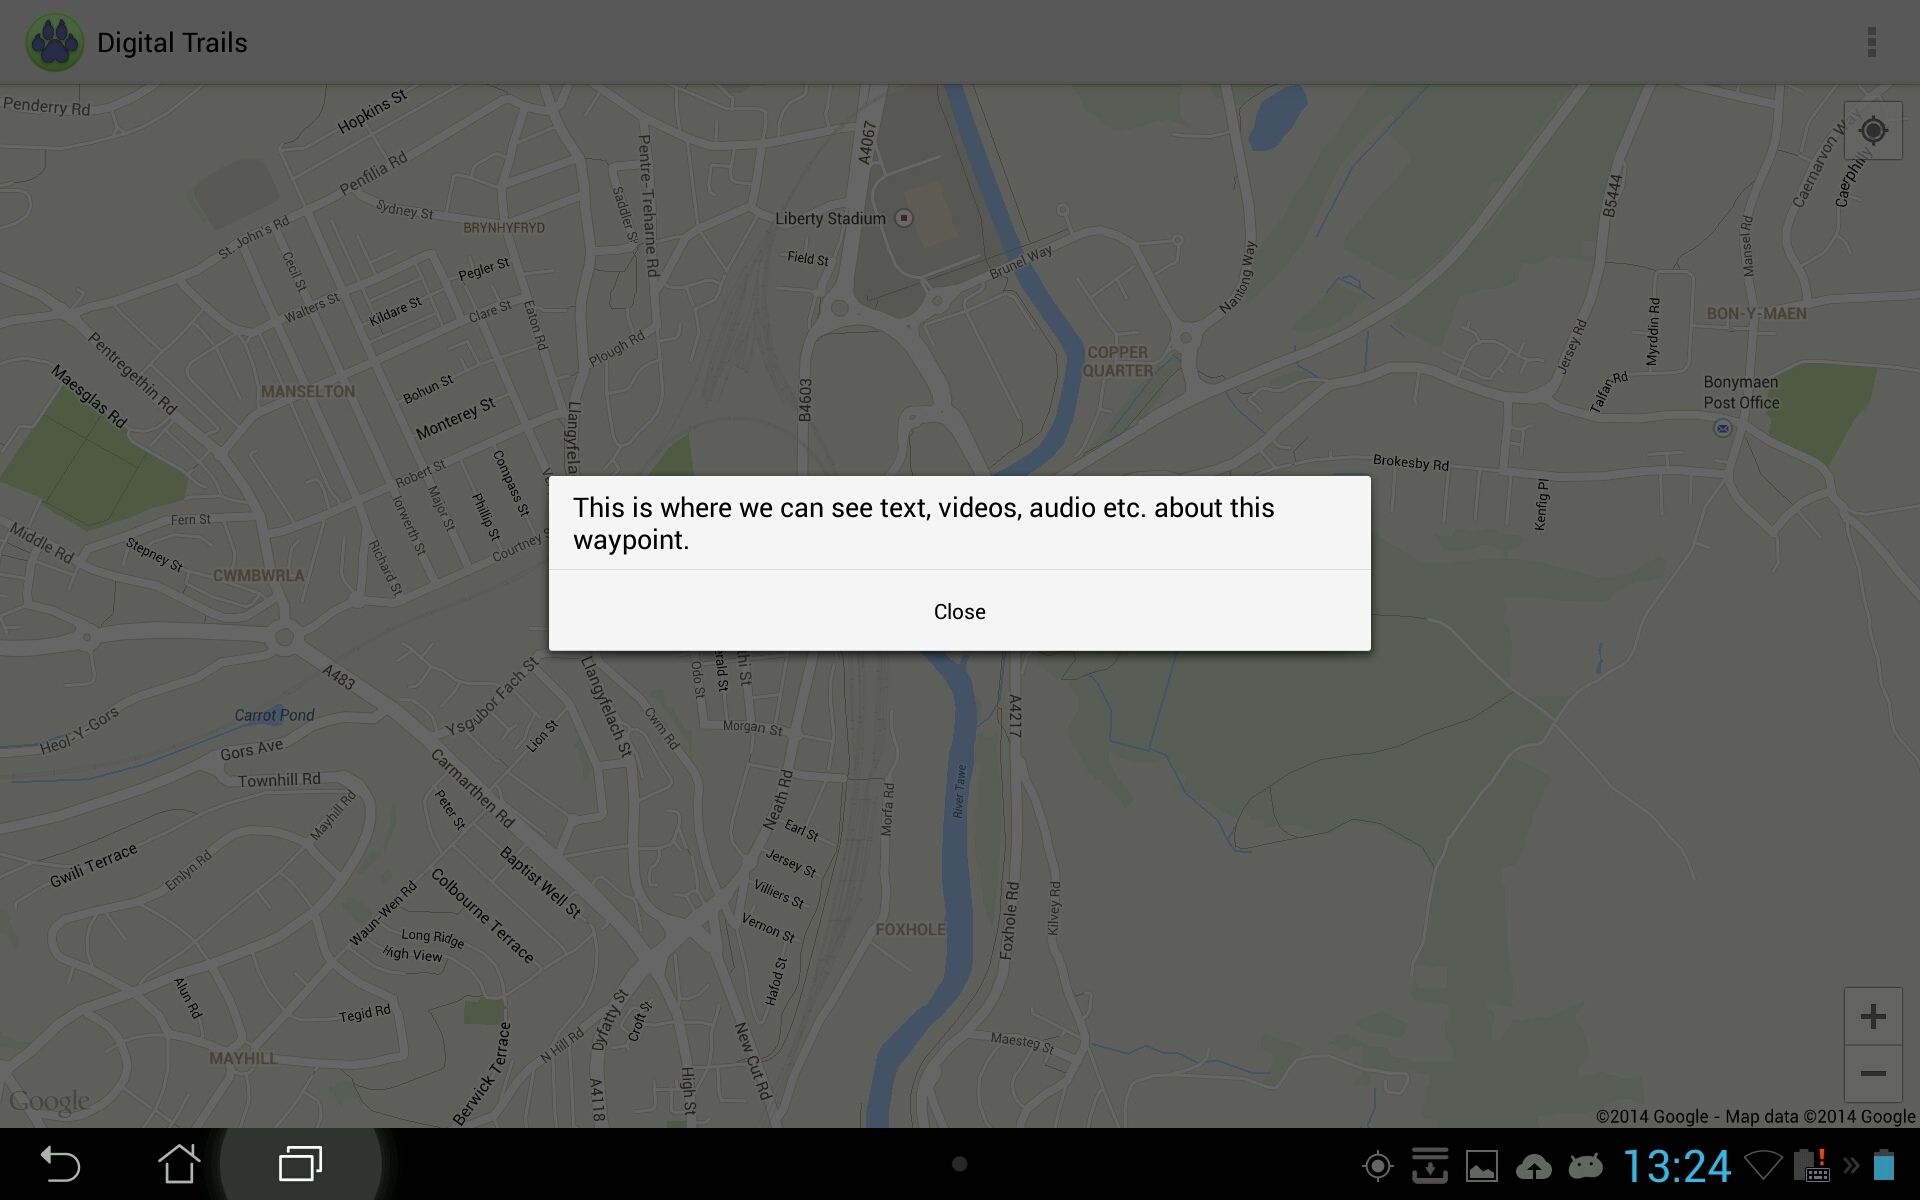
\includegraphics[angle=90, width=.6\linewidth]{wpInfoDialog.jpg}
\caption{Screenshot of the MapActivity Information Dialog.}
\label{fig:wpInfoDialog}
\end{figure}

Users may also change the style of the map to ``Normal'', ``Hybrid'' or ``Satellite''; rotate, zoom, pan and tilt the map with gestures and zoom the map in and out and find the user's current location with on-screen buttons. These can be see in Figures~\ref{fig:mapOptions} and~\ref{fig:userLocation}.

\begin{figure}[H]
\centering
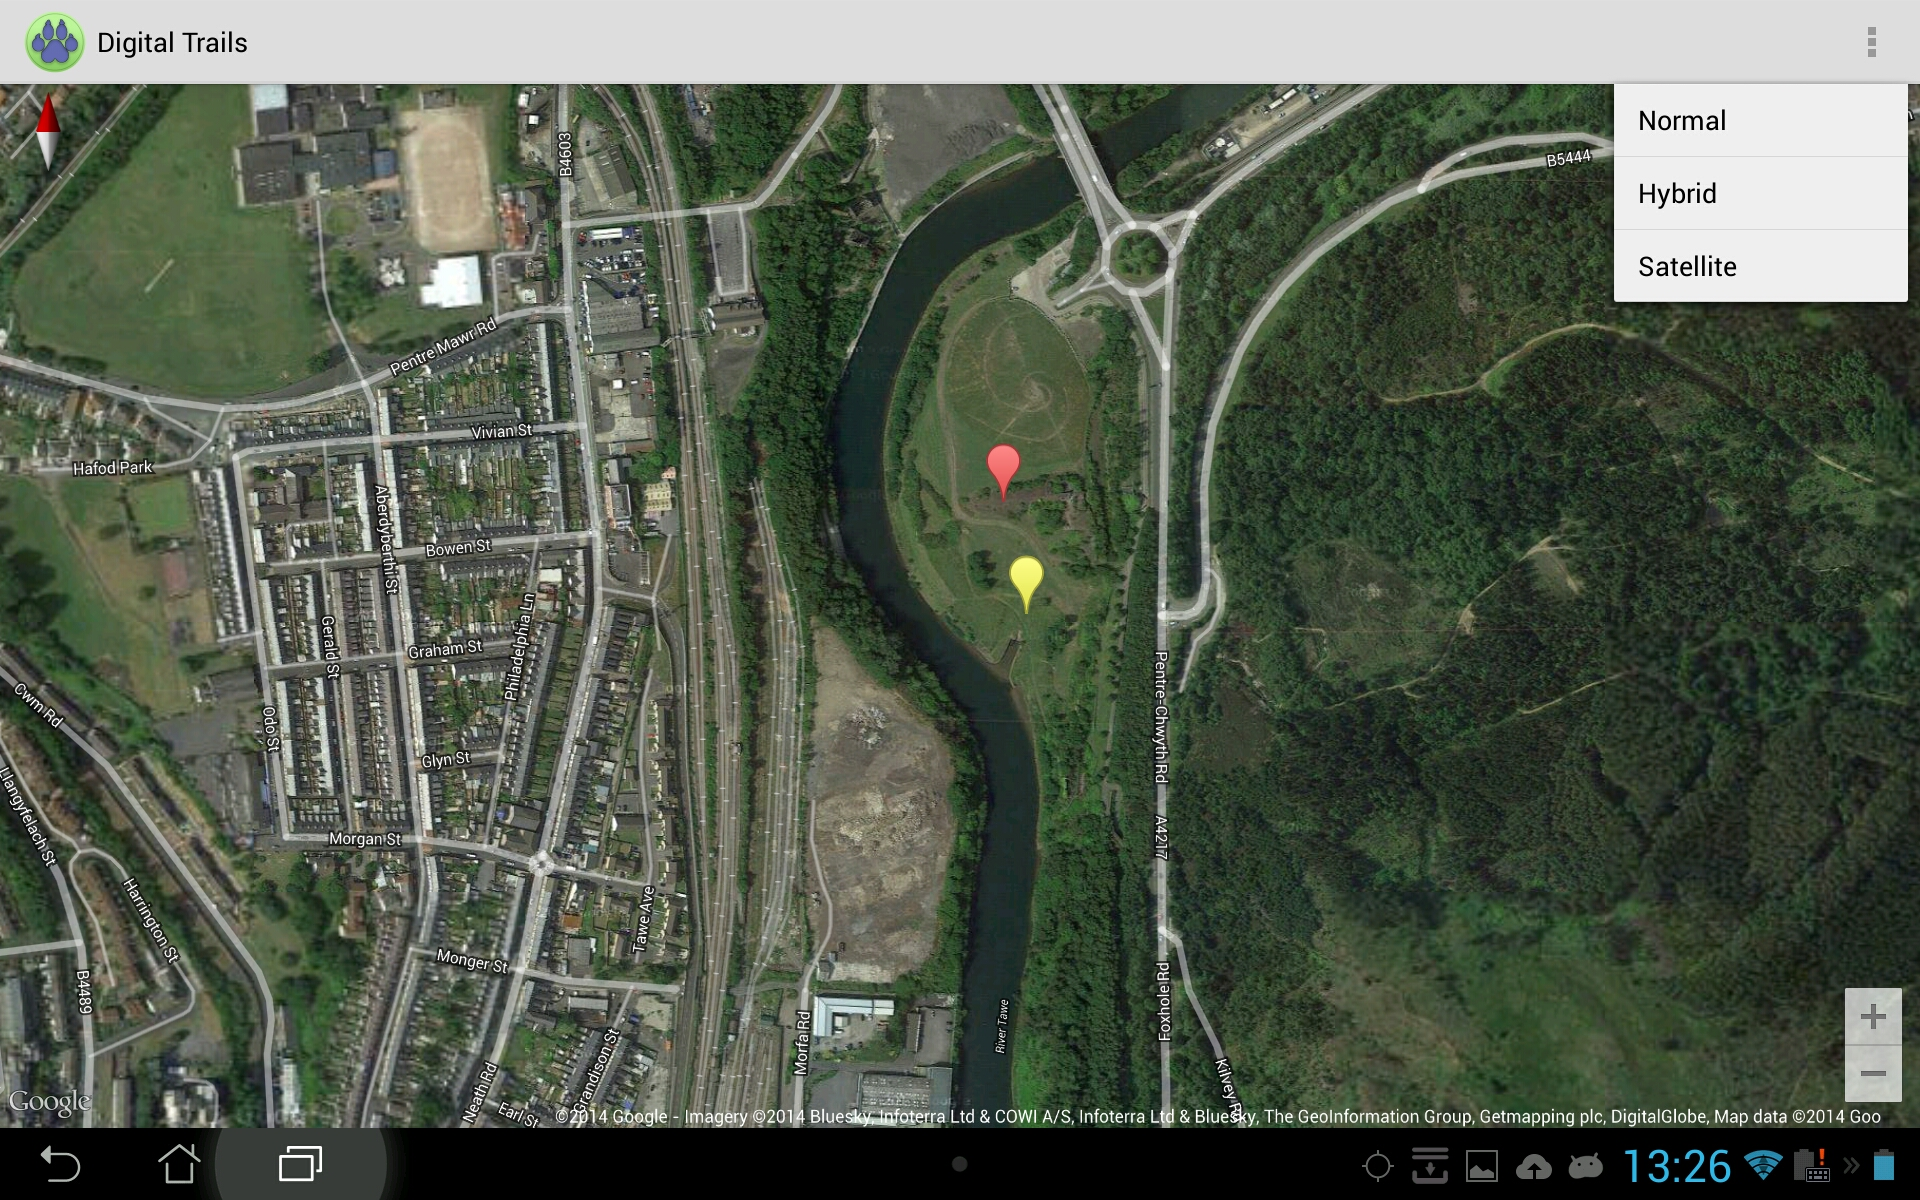
\includegraphics[angle=90, width=.6\linewidth]{mapOptions.jpg}
\caption{Screenshot of the MapActivity map options.}
\label{fig:mapOptions}
\end{figure}

\begin{figure}[H]
\centering
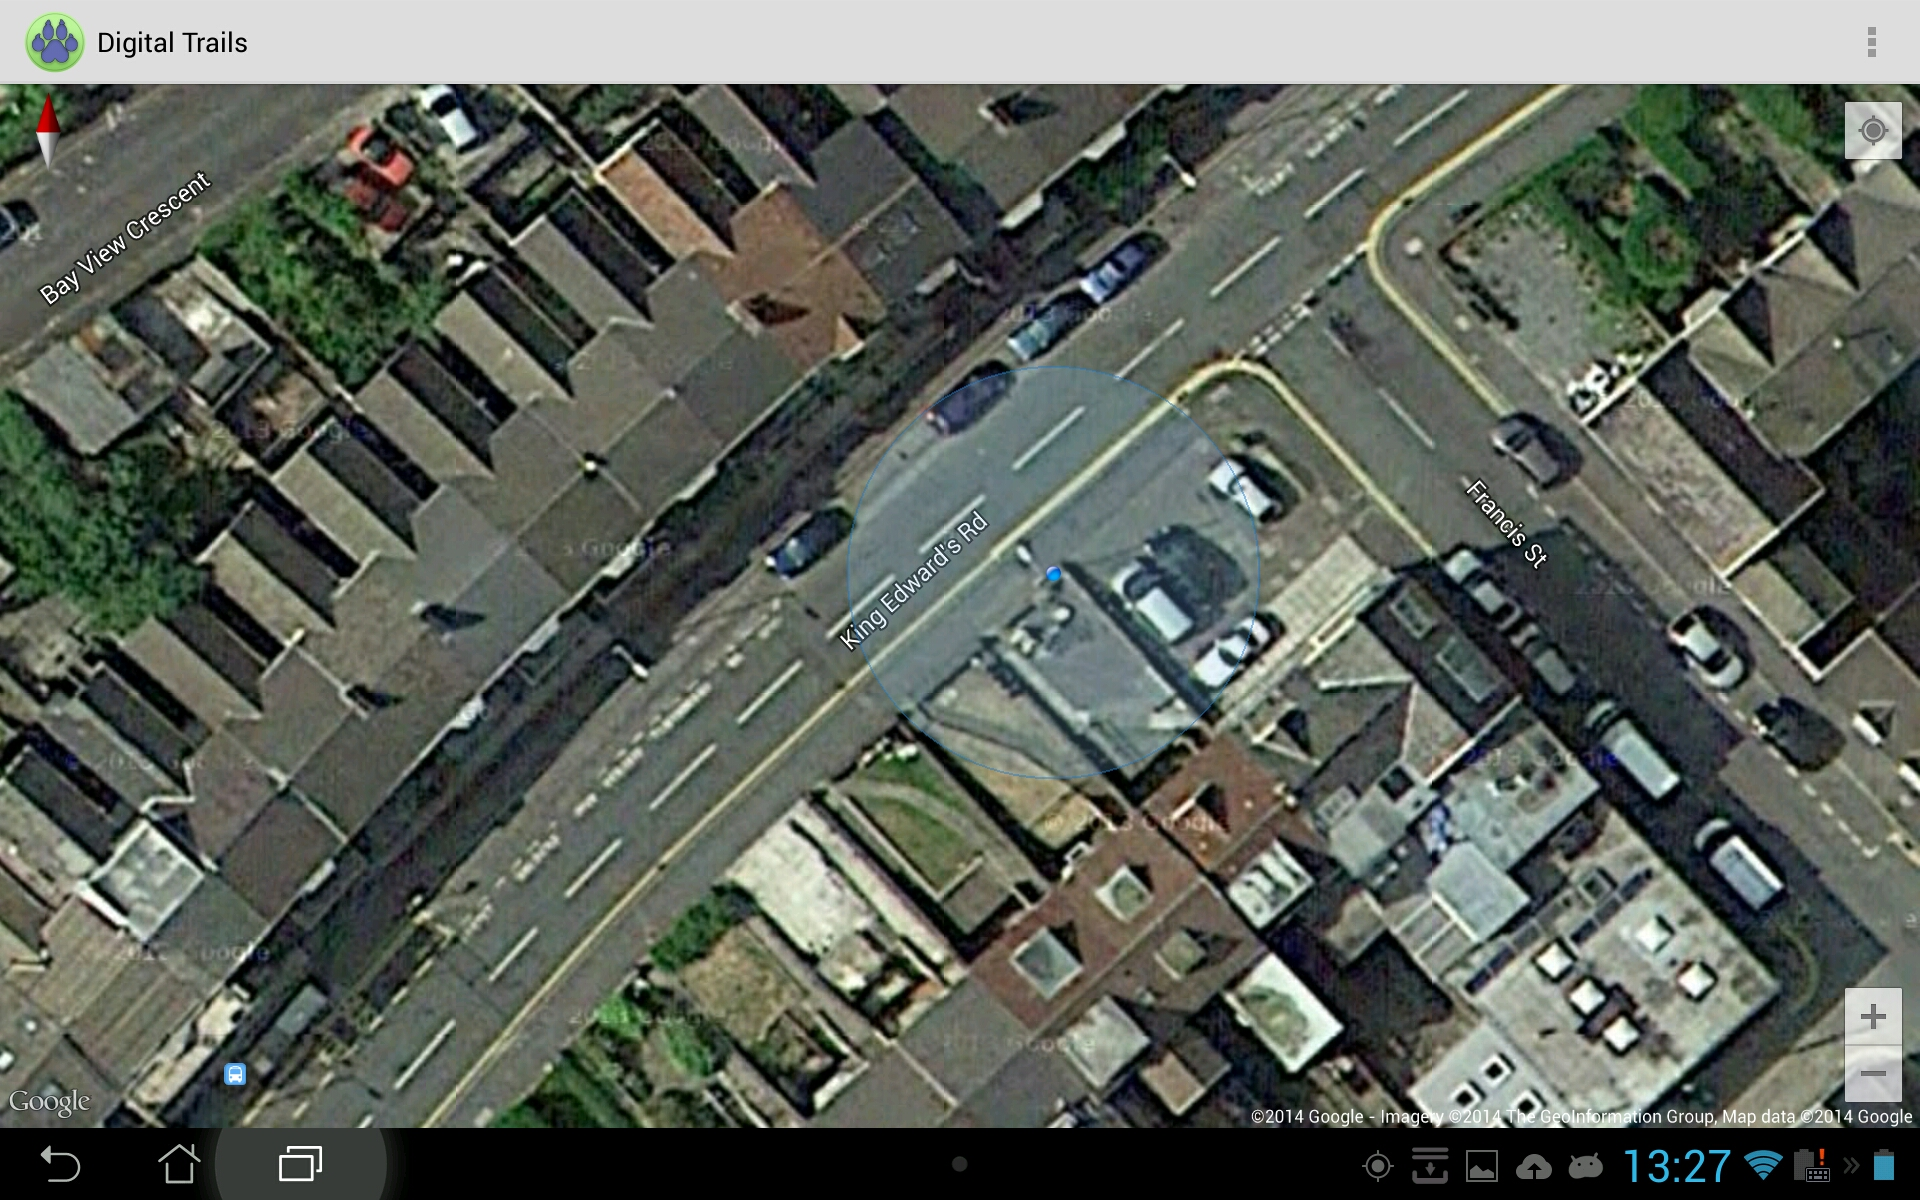
\includegraphics[angle=90, width=.6\linewidth]{userLocation.jpg}
\caption{Screenshot of the MapActivity displaying user's current location.}
\label{fig:userLocation}
\end{figure}

Future development includes creating a custom InfoWindowAdapter for the InfoWindow, allowing for more customisable data to be displayed. The next waypoint to visit shall be displayed in a different colour than the other waypoints, whilst previously visited waypoints will also change colour. 


\subsection{Authorisation}
\label{sec:authorisation}

\subsection{Fragments}
\label{sec:fragments}
%- Authorisation
%- Google Maps
%- Current design to sync with server
%- Chris can chuck in his Fragments here, so he has some code to show.

\subsection{Web Portal}

\subsubsection{API}
\subsubsection{Web Application}
\subsubsection{Object Relation Mapper}

\section{Programming Guidelines}
%- I'll write android guidelines.
%- Adam/Tom get on the web guidelines.

\section{Risk Analysis Review}
%- Explain risks we dealt with, cross reference to our initial table.
%- Add new risks that arose (Poor work environment, lab computers suck, hudl broken, hudl missing USB driver - not supported as a dev. device).

\section{Project Schedule Review}
%- What sprints we have completed.
%- What reqs / specifications are completed Chris Lewis' favourite job!).
%- Are we ahead or behind schedule? (hard for us to answer)
%- Did we have to modify any requirements / specs to get this far? Did we add any or drop any?
%- Create new gantt chart and compare it with the initial one.
%- Update online sprint software, make it look like we completed sprints on time.
%- Client feedback so far, previous client meetings, planned meetings, launch event we attended etc.

\section{Summary}
%- What we have planned next, I guess.

%References as subsection
\newpage
\bibliographystyle{plain}
\bibliography{bibliography}
\end{document}